%!TEX root = main.tex

%\begin{itemize}
%\item Show the convergence rate of SGD something like
%\[
%f(\x_T) - f^* \leq \Theta\left({L\over T} + {\sum_{t=1}^T \E\|\g_t^{(full)} - \nabla f(\x_t)\|^2/T \over \sqrt{T}}\right) 
%\]
%and emphasize two things: 1) the unbiased stochastic gradient is required for convergence; and 2) the key to improve the convergence is to reduce the variance of stochastic gradient.
%\item Using naive quantization does not work as shown in Section 2.1, since it is biased.
%\item Using the proposed double sampling can ensure unbiased sampling, that is, $\E(\g_t) = \nabla f(\x_t)$ and the stochastic variance of using double sampling can be estimated by
%\begin{align*}
%\E\left[\|\g_t - \nabla f(\x_t)\|^2\right] \leq &\underbrace{\E \|\g_t^{(full)}- \nabla f(\x_t)\|^2}_{\text{from the standard stochastic gradient variance}}
%\\
%&+ \underbrace{\E\|\g_t - \g_t^{(full)}\|^2}_{\text{from the quantization}}
%\end{align*}
%Key point: 1) the first term cannot be avoid and the second term is due to using quantization; 2) in order to not degrade the convergence rate, need to make sure the second term is comparable to the first term. 
%\item Estimate the second term by something like
%\begin{align*}
%&\E\|\g_t - \g_t^{(full)}\|^2 \leq \\
%&\Theta\left(\mathcal{TV}(\a_t) (\mathcal{TV}(\a_t)\|\x\odot \x\| + \|\a_t^\top \x\|^2 + \|\x\odot \x\|\|\a_t\|^2)\right)
%\end{align*}
%where the total variance is 
%\[
%\mathcal{TV}(\a_t) := \E \|Q(\a_t) - \a_t\|^2
%\]
%\item Estimate the upper bound of $\mathcal{TV}(\a_t)$ by something like $n/s^2$ (maybe using uniform quantization), which basically suggests the conclusion in Corollary 1.
%\item In the meantime, we can perform the optimal quantization (not necessarily uniform) to minimize the empirical total variance or mean variance equivalently 
%\[
%\mathcal{TV}(\a_t) = n\mathcal{MV}(\a_t),
%\]
%which is shown in Section 3.
%\end{itemize}


\vspace{-0.5em}
In this section, we focus on linear models with possibly non-smooth regularization. We have labeled data points $(\a_1, b_1), (\a_2, b_2), \ldots, (\a_K, b_K) \in \R^n \times \R$, and our goal is to minimize the function
\vspace{-0.5em}
\begin{align}
F(\x) = \underbrace{\frac{1}{K} \sum_{k = 1}^K \| \a_k^\top \x - b_k \|_2^2}_{=: f(\x)} + R(\x) \; ,
\label{eq:linear}
\end{align}
i.e., minimize the empirical least squares loss plus a non-smooth regularization $R(\cdot)$ (e.g., $\ell_1$ norm, $\ell_2$ norm, and constraint indicator function). SGD is a popular approach for solving large scale machine learning problems. It works as follows: at step $\x_t$, given an unbiased gradient estimator $\g_t$, that is, 
$\E(\g_t) = \nabla f(\x_t),$
we update $\x_{t+1}$ by
\[
\x_{t+1} = \text{prox}_{\gamma_t R(\cdot)}\left( \x_t - \gamma_t \g_t\right)
\]
where $\gamma_t$ is the predefined step length. SGD guarantees the following convergence property:
\begin{theorem}\label{thm:sgd-conv}[e.g., \cite{2014arXiv1405.4980B}, Theorem 6.3]
Let the sequence $\{\x_t\}_{t=1}^T$ be bounded. Appropriately choosing the steplength,% (e.g., $\gamma_t = 1 / ( L + \sqrt{T})$), 
we have the following convergence rate for \eqref{eq:linear}
% 
%Let $\mathcal{X} \subseteq \R^n$ be convex, and let $f: \mathcal{X} \to \R$ be an unknown, convex, and $L$-smooth. Let $\x_0 \in \mathcal{X}$ be given, and let $R^2 = \sup_{\x \in \mathcal{X}} \| \x - \x_0 \|^2$. Suppose we run projected SGD on $f$ with access to independent stochastic gradients with variance bound $\sigma^2$ for $T$ steps, with step size $\eta_t = 1 / ( L + \gamma^{-1})$, where $\gamma = \frac{R}{\sigma} \sqrt{\frac{2}{T}}$, and
\begin{equation}
F\left(\frac{1}{T} \sum_{t = 0}^T \x_t\right) - \min_{\x}F(\x) \leq \Theta\left({1\over T} + {\sigma \over \sqrt{T}}\right) 
\label{eq:sgd-conv}
%T = O \left( R^2 \cdot \max \left( \frac{2 \sigma^2}{\epsilon^2} , \frac{L}{\epsilon} \right) \right).
\end{equation}
where $\sigma$ is the upper bound of the mean variance 
\[
\sigma^2 \geq {1\over T}\sum_{t=1}^T \E\|\g_t - \nabla f(\x_t)\|^2. 
\]
%Then $\E \left[ f \left( \frac{1}{T} \sum_{t = 0}^T \x_t \right) \right] - \min_{\x \in \mathcal{X}} f(\x) \leq \epsilon$.
\end{theorem} 
\vspace{-2em}
There are three key factors to ensure for SGD:
\begin{enumerate}
\vspace{-0.75em}
\item Computing stochastic gradient $\g_t$ is cheap;
\vspace{-0.75em}
\item The stochastic gradient $\g_t$ should be unbiased;
\vspace{-0.75em}
\item The stochastic gradient variance $\sigma$ dominants the convergence efficiency, so it needed to be controlled appropriately.
\end{enumerate}
\vspace{-1.5em}
The common choice is to uniformly select one sample:
\vspace{-0.5em}
\begin{align}
\g_t = \g_t^{(full)} := \a_{\pi(t)} (\a_{\pi(t)}^\top \x - b_{\pi(t)})
\label{eq:sgfull}
\end{align} 
($\pi(t)$ is a uniformly random integer from $1$ to $K$). We abuse the notation and let $\a_t = \a_{\pi(t)}$. Note that $\g_t^{(full)}$ is an unbiased estimator $\E [\g_t^{(full)}] = \nabla f(\x_t)$. Although it has received success in many applications, 
if the precision of sample $\a_{t}$ can be further decreased,
we can save, potentially one order of magnitude, bandwidth
of reading $\a_{t}$ (e.g., in sensor networks) and the associated computation (e.g.,
each register can hold more numbers). 
This motivates us to use low precision sample points to train the model. The following will introduce the proposed low precision SGD framework by meeting all three factors for SGD.


%\paragraph*
\vspace{-0.5em}
\subsection{Stochastic Quantization for Saving Bandwidth} 
\vspace{-0.5em}

We propose to use the stochastic quantization to generate a low precision version of an arbitrary vector $\v$ in the following 
way. Given a vector
$\v$, let $M(\v)$ be a scaling factor such that $-1 \le \v/M(\v) \le 1$. Without loss of generality, let $M(\v)=||\v||_2$. We partition the interval $[-1, 1]$ using $s+1$ separators: $-1 = l_0 \le l_1 ... \le l_{s} = 1$; for each number $v$ in $\v/M(\v)$, we 
quantize it to one of two nearest separators: $l_i \le v \le l_{i+1}$. We denote the \emph{stochastic quantization} function by $Q(\v, s)$ and choose the probability of quantizing to different separators such that $\E[Q(\v, s)] = \v$. We use $Q(\v)$ when $s$ is not relevant.

\vspace{-0.5em}
\subsection{Double Sampling for Unbiased Stochastic Gradient}
\vspace{-0.5em}
%\subsection
%\paragraph{Naive Stochastic Quantization does not Work}

\begin{wrapfigure}{r}{0.23\textwidth}
  \begin{center}
    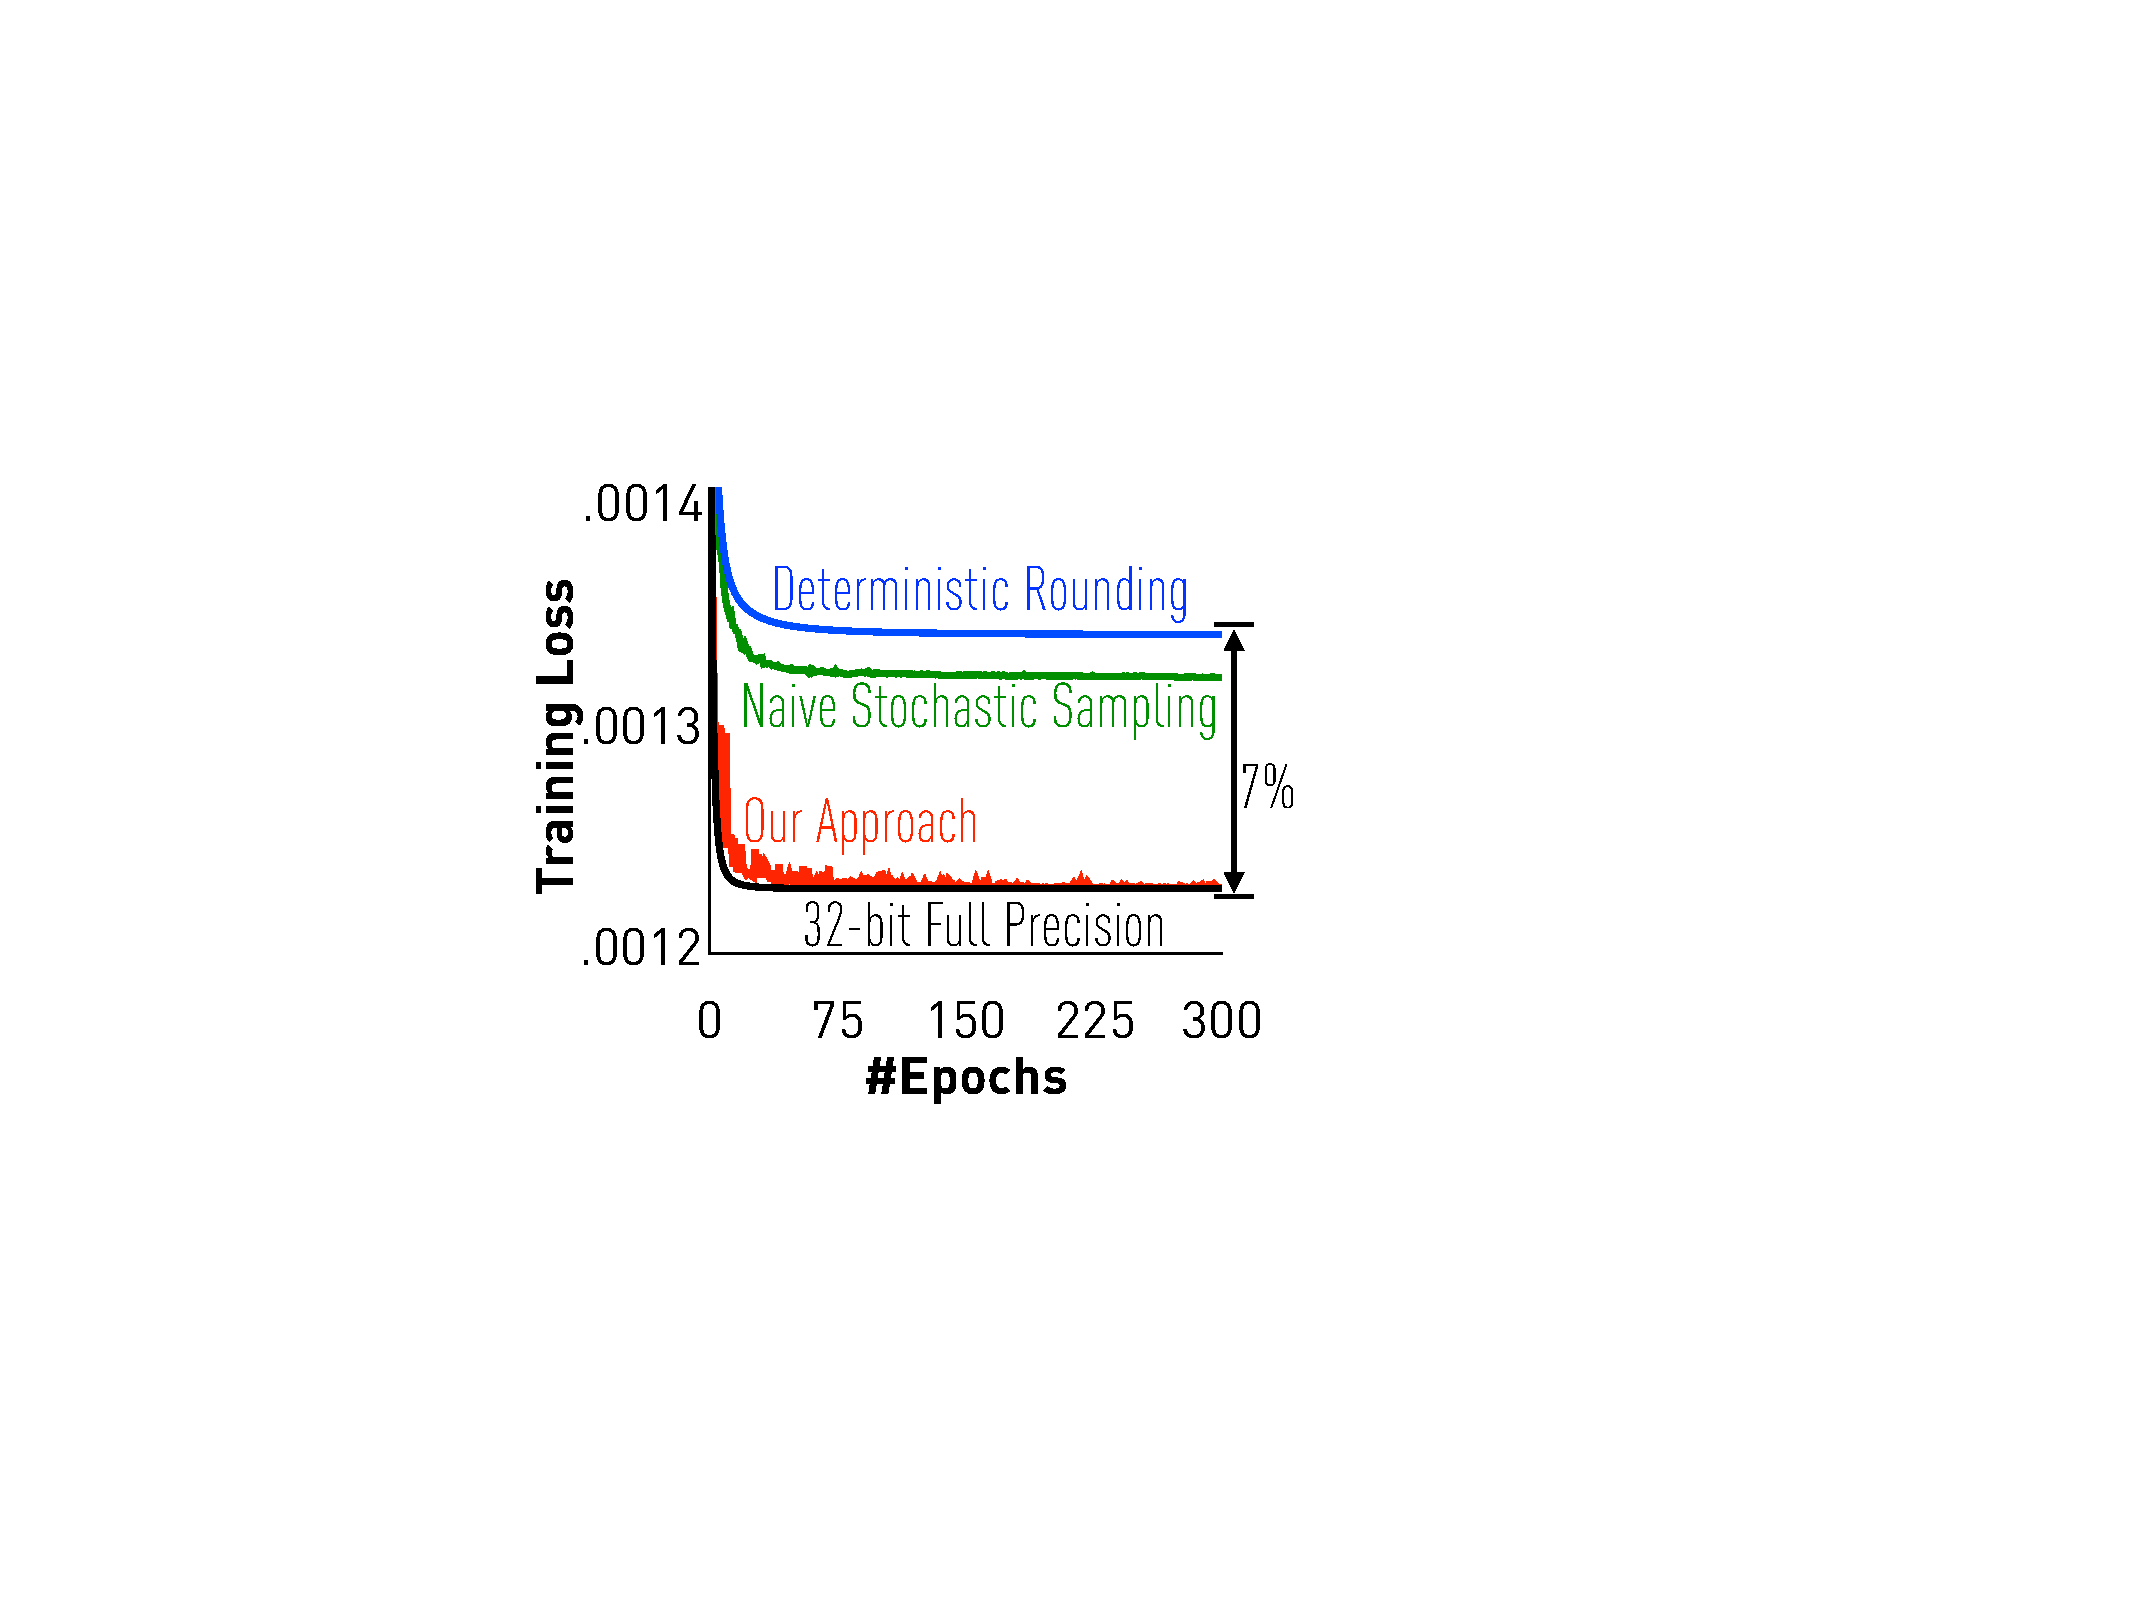
\includegraphics[width=0.23\textwidth]{micro-experiments/gap.pdf}
  \end{center}
  \label{fig:gap}
\end{wrapfigure}
The naive way to use low precision samples $\hat{\a}_t := Q(\a_t)$ is 
\[
\hat{\g}_t := \hat{\a}_t \hat{\a}_t^\top \x - \hat{\a}_t b_t.
\]
However, \emph{the naive approach does not work} (does not guarantee convergence), because it is biased: 
\[
\E[\hat{\g}_t] := \a_t \a_t^\top \x - \a_t b_t + D_{\a} \x, 
\]
where $D_{\a}$ is diagonal and its $i$th diagonal element is 
\[
\E[ Q(\a_i)^2 ] - \a_i^2.
\]
%
%\vspace{-0.5em}
%We focus on quantizing the input samples.
%We first establish that, when we quantize $\a_t$
%using the stochastic quantization methods designed
%for gradient, it introduces significant bias.
%Let $\hat{\a}_t = Q(\a_t)$ be the quantized
%sample, the gradient becomes
%\[
%\g_t := \hat{\a}_t \hat{\a}_t^\top \x - \hat{\a}_t b_t.
%\]
%It is not hard to see that the expected gradient is: 
%\[
%\E[\g_t] := \a_t \a_t^\top \x - \a_t b_t + D_{\a} \x, 
%\]
%where $D_{\a}$ is diagonal and its $i$th diagonal element is 
%\[
%\E[ Q(\a_i)^2 ] - \a_i^2.
%\]
%\todo{y axis here is weird}


\vspace{-0.5em}
Since $D_{\a}$ is non-zero, we obtain a \emph{biased} estimator of the gradient, so the iteration is unlikely to converge. 
The figure on the right illustrates the bias caused by a non-zero $D_{\a}$. In fact, it is easy to see that in instances where the minimizer $\x$ is large and gradients become small, we will simply diverge. 

%\vspace{-0.5em}
%\subsection{Double Sampling}
%\vspace{-0.5em}
%\paragraph{Double Sampling}
We now present a simple method to fix the biased gradient estimator. We generate two independent random quantizations and revise the gradient:
\begin{align}
\g_t := Q_1 (\a_t) (Q_2 (\a_t)^\top \x + b_t) \; .
\label{eq:double}
\end{align}
This gives us an unbiased estimator of the gradient. 

\paragraph*{Overhead of Storing Two Samples}
The astute reader will have noticed that one implication of double sampling is the overhead of sending
two samples instead of one. We note that this will not introduce $2\times$
overhead in terms of data communication. Instead, just one additional bit
is needed the second sample, because of correlation, as the two samples 
differ by at most one bit. More generally, since samples
are used symmetrically, sending $k$ samples only requires $\log_2 k$ more bits.

\vspace{-0.5em}
\subsection{Variance Reduction}
\vspace{-0.5em}

From Theorem~\ref{thm:sgd-conv}, the mean variance ${1\over T}\sum_{t}\E\|\g_t - \nabla f(\x)\|^2$ will dominate the convergence efficiency. It is not hard to see that the variance of the double sampling based stochastic gradient in \eqref{eq:double} can be decomposed into
\vspace{-0.5em}
\begin{align*}
\E\|\g_t - \nabla f(\x_t)\|^2 & \leq \E \|\g_t^{(full)}- \nabla f(\x_t)\|^2 
\\
&+ \E \|\g_t - \g_t^{(full)})\|^2
\end{align*}
The first term is from the full stochastic gradient, which can be reduced by using strategies such as mini-batch, weight sampling, etc. Reducing the first term is issue orthogonal to this paper. 
Rather, we are interested in the second term, which is the additional cost of using low precision samples. All strategies for reducing the variance of the first term can seamlessly combine with the approach of this paper. 
The additional cost can be bounded by
\begin{lemma} 
The stochastic gradient variance using double sampling in \eqref{eq:double} $\E\|\g_t - \g_t^{(full)}\|^2$ can be bounded by
\begin{align*}
%&\E\|\g_t - \g_t^{(full)}\|^2 \leq \\
&\Theta\left(\mathcal{TV}(\a_t) (\mathcal{TV}(\a_t)\|\x\odot \x\| + \|\a_t^\top \x\|^2 + \|\x\odot \x\|\|\a_t\|^2)\right).
\end{align*}
where $\mathcal{TV}(\a_t) := \E\|Q(\a_t) - \a_t\|^2$ and $\odot$ denotes the elementwise product.
\end{lemma}
Thus minimizing $\mathcal{TV}(\a_t)$ is key for reducing variance. 

\vspace{-0.5em}
\paragraph{Uniform quantization} Intuitively, more levels of quantization, the lower the variance. The following result makes this quantitative dependence precise. 
%We assume that these separators are uniformly distributed, and revisit this in Section~\ref{sec:optimal}.
%We have~\cite{Alistarh:2016:ArXiv}: 
\begin{lemma}
\label{lem:quant-facts} [\cite{Alistarh:2016:ArXiv}]
Assume that quantization levels are uniformly distributed. For any vector $\vec{v} \in \R^n$, we have that $\E [Q (\vec{v},s)] = \vec{v}$. Further, the total variance using uniform quantization with  $s$ levels is bounded by
\[
\mathcal{TV}_s(\v):=\E [\| Q (\vec{v},s) - \v\|_2^2] \leq \min( n/s^2,\sqrt{n}/s)) \| \vec{v} \|_2^2. \;
\]
\end{lemma} 

\vspace{-1em}
Hence, the stochastic gradient variance of double sampling is bounded by
\[
\E\|\g_t - \nabla f(\x_t)\|^2 \leq \sigma^2_{(full)} + \Theta \left( {n /s^2} \right)
\]
where $\sigma^2_{(full)} \geq \E \|\g_t^{(full)} - \nabla f(\x)\|^2$ is the upper bound of using full stochastic gradient, assuming that $\x$ and all $\a_k$'s are bounded. Because the quantization level $s$ is exponential to the number of bits, to ensure these two terms are comparable (using low precision sample does not degrade the convergence rate), the number of bits only needs to be greater than $\Theta (\log n /\sigma_{(full)})$: Even for linear models with millions
of features, 32-bits is likely to be  ``overkill.''

\vspace{-0.5em}
The uniform quantization provides us an intuitive dependence between variance and the level of quantization. However, in practice, we can do better by designing the optimal quantization separation given the quantization level $s$. This motivates
our study in the next section.
 

%\vspace{-0.5em}
%\paragraph{Variance}
%
%Let $r = r(s) = 1 + \min (n / s^2, \sqrt{n}/ s)$ be the blow-up in the second moment because of quantization:
%\begin{lemma}
%\label{lem:qbound}
%    Given $\a_k, \x, b_k$, suppose $\| \a_k \|_2^2 \leq A^2, \| \x \|_2^2 \leq R^2$ and $\max_i |\a_k| \leq M_a$.
%    Let $\g_k^{(full)}$ be the unquantized stochastic gradient. We have
%    \[
%    \E_{Q_1, Q_2} [\| \g_k \|_2^2] \leq r \cdot \left( \| \g_k^{(full)} \|_2^2 \cdot \frac{M_a^2}{\| \a_k \|_2^2} + \frac{A^2 M_a^2 R^2}{s^2} \right)\; .
%    \]
%\end{lemma}
%
%This implies the following variance bound:
%\begin{corollary}
%    Let $\a_k, \x, b_k, \g_k^{(full)}$ be as above.
%    Suppose $\E [\| \g_k^{(full)} - \nabla f(\x_k) \|_2^2 ] \leq \sigma^2$ and $\E [\| \g_k^{(full)} \|_2^2] \leq B$. We have
%    \[
%    \E \left[ \| \g_k - \nabla f(\x_k) \|_2^2 \right] \leq  \sigma^2 + \left(r \frac{M_a^2}{\| \a_k \|_2^2} - 1\right) B + \frac{r A^2 M_a^2 R^2}{s^2} \; ,
%    \]
%    where the expectation is taken over $\g_k^{(full)}$ and the randomness of the quantization.
%\end{corollary}
%
%This corollary suggests that the quantized stochastic gradient variance is bounded by
%\[
%\E \left[ \| \g_k - \nabla f(\x_k) \|_2^2 \right] \leq \sigma^2 + \Theta(n/s^2) \;
%\]
%in the scenario when $M_i (\vec{v}) = \| \vec{v} \|_2 $.
%The first term $\sigma^2$ is introduced by stochastic gradient, while the second term is introduced by quantization. Because the value of $s$ is 
%exponential to the number of bits, to ensure these two terms are comparable (to maintain the same convergence rate), the number of bits needs to be greater than $\Theta(\log n / \sigma)$. We see that even for linear models with millions
%of features, 32-bits is likely to be  ``overkill.''
%
%
%
%\vspace{-0.5em}
%\paragraph*{Overhead of Storing Two Samples}
%One system implication of double sampling is the overhead of sending
%two samples instead of one. We note that this will not introduce $2\times$
%overhead in terms of data communication, instead, just a single more bit
%for the second sample because of the correlation (these two samples 
%are only different by at most one bit). More generally, because samples
%are used symmetrically, sending $k$ samples only require $\log_2 k$ more bits.
%
%\vspace{-0.5em}
%\paragraph*{Extensions}
%
%All of our results can be applied to 
% problems 
%with possibly non-smooth regularization term. The key substitution is to use the proximal update defined in \eqref{eq:proxupdate}.
%Also, extending our result to least-squares SVMs for classification is trivial~\cite{Suykens:1999:Book}.
%We leave these details to the full version
%of this paper.
%
%\vspace{-0.5em}
%\subsection{End-to-end Quantization}
%\vspace{-0.5em}
%
%We can now develop an end-to-end quantization strategy that
%quantizes gradients, model, and input samples all 
%at the same time. The gradient becomes:
%\[
%\g_k := Q_1 \left( Q_2(\a_k, s ) ( Q_3(\a_k, s)^\top Q_4(\x, s) + b_k) , s \right),
%\]
%\noindent 
%where all $Q$'s are independent quantizations.
%
%%  $Q_3$ and 
%%The iteration becomes: 
%%
%%\begin{eqnarray}
%%	\x = \x - \gamma \g_k.
%%\end{eqnarray}
%
%\noindent From combining the previous results, we have:
%
%\begin{corollary}
%    \label{cor:full-quantization}
%    Let $\a_k, \x, b_k$ be so that $\| \a_k \|_2^2 \leq 1, \| \x \|_2^2 \leq R^2$.
%    Let $M_a, M_x$ be as above, and let $\g_k^{(full)}$ be the (unquantized) stochastic gradient.
%    We have
%    \[
%    \E [\| \g_k \|_2^2] \leq r^2 M_a \cdot \left(  \| \g_k^{(full)} \|_2^2 + \frac{R^2}{s^2}   + \frac{r M_a R^2}{s^2} \right) \; .
%    \]
%\end{corollary}




